\documentclass[aspectratio=169,10pt]{beamer}

\usetheme{Madrid}
\usecolortheme{seahorse}
\setbeamertemplate{footline}[frame number]

\usepackage{amsmath}
\usepackage{amssymb}
\usepackage{amsfonts}
\usepackage{graphicx}
\usepackage{listings}
\usepackage{xcolor}
\usepackage{multicol}
\usepackage{hyperref}

\graphicspath{{figures/}}

% Listing style
\lstset{
    basicstyle=\ttfamily\scriptsize,
    numbers=left,
    numberstyle=\tiny\color{gray},
    keywordstyle=\color{blue},
    commentstyle=\color{green!50!black}\itshape,
    stringstyle=\color{red},
    breaklines=true,
    frame=single,
    language=Python
}

\title[Chapter 9a: Approximating Solutions]{Chapter 9a: Approximating Solutions \\Applications of Fixed Point Theorems}
\author{Pathak}
\date{\today}
\institute{Nonlinear Analysis and Fixed Point Theory}

\begin{document}

\frame{\titlepage}

\begin{frame}{Overview}
    \tableofcontents
\end{frame}

% ============================================================================
\section{9.1: Application to Geometry of Banach Spaces}
% ============================================================================

\begin{frame}{Banach Spaces: Foundational Results}
    \begin{block}{Lemma 9.1}
        Let $T$ be locally quasi-nonexpansive at $p \in \tilde{\mathcal{F}}(T)$ w.r.t. $\{x_n\}$, and
        \[\lim_{n \to \infty} d(x_n, \tilde{\mathcal{F}}(T)) = 0\]
        Then, $\{x_n\}$ is a Cauchy sequence.
    \end{block}

    \vspace{0.3cm}

    \begin{block}{Theorem 9.3 (Pathak)}
        Let $\tilde{\mathcal{F}}(T)$ be a nonempty closed set. Then:
        \begin{enumerate}
            \item $\displaystyle \lim_{n \to \infty} d(x_n, \tilde{\mathcal{F}}(T)) = 0$ if $\{x_n\}$ converges to $p \in \tilde{\mathcal{F}}(T)$;
            \item $\{x_n\}$ converges to a point in $\tilde{\mathcal{F}}(T)$ if $\displaystyle \lim_{n \to \infty} d(x_n, \tilde{\mathcal{F}}(T)) = 0$, $T$ is locally quasi-nonexpansive at $p \in \tilde{\mathcal{F}}(T)$ w.r.t. $\{x_n\}$, and $X$ is complete.
        \end{enumerate}
    \end{block}

    \vspace{0.3cm}
    These results provide convergence guarantees in Banach spaces.
\end{frame}

\begin{frame}{Theorem 9.4: Geometry and Approximation}
    \begin{block}{Theorem 9.4 (Pathak)}
        Let $C$ be a closed subset of Banach space $X$, let $z \in X \setminus C$, and let $K = K(z,r)$ be a closed ball with radius $r = d(z,C) = R$. Let $x$ be arbitrary in $C$, let $\{x_n\}$ be a sequence in $C$ converging to $x$, and let $T: C \to X$ be continuous with $T(x_n) \in C \cap \mathcal{D}(x,K)$ for each $n \in \omega$. Then:
        \begin{enumerate}
            \item $\displaystyle \lim_{n \to \infty} d(x_n, \tilde{\mathcal{F}}(T)) = 0$ if $\{x_n\}$ converges to a point $p \in F(T)$;
            \item $\{x_n\}$ converges to a point in $\tilde{\mathcal{F}}(T)$ if $\displaystyle \lim_{n \to \infty} d(x_n, \tilde{\mathcal{F}}(T)) = 0$ and $T$ is locally quasi-nonexpansive at $p \in \tilde{\mathcal{F}}(T)$ w.r.t. $\{x_n\}$.
        \end{enumerate}
    \end{block}

    \vspace{0.3cm}
    This geometric approach provides a bridge between fixed point theory and approximation in Banach spaces.
\end{frame}

\begin{frame}{Geometric Visualization}
    \begin{center}
        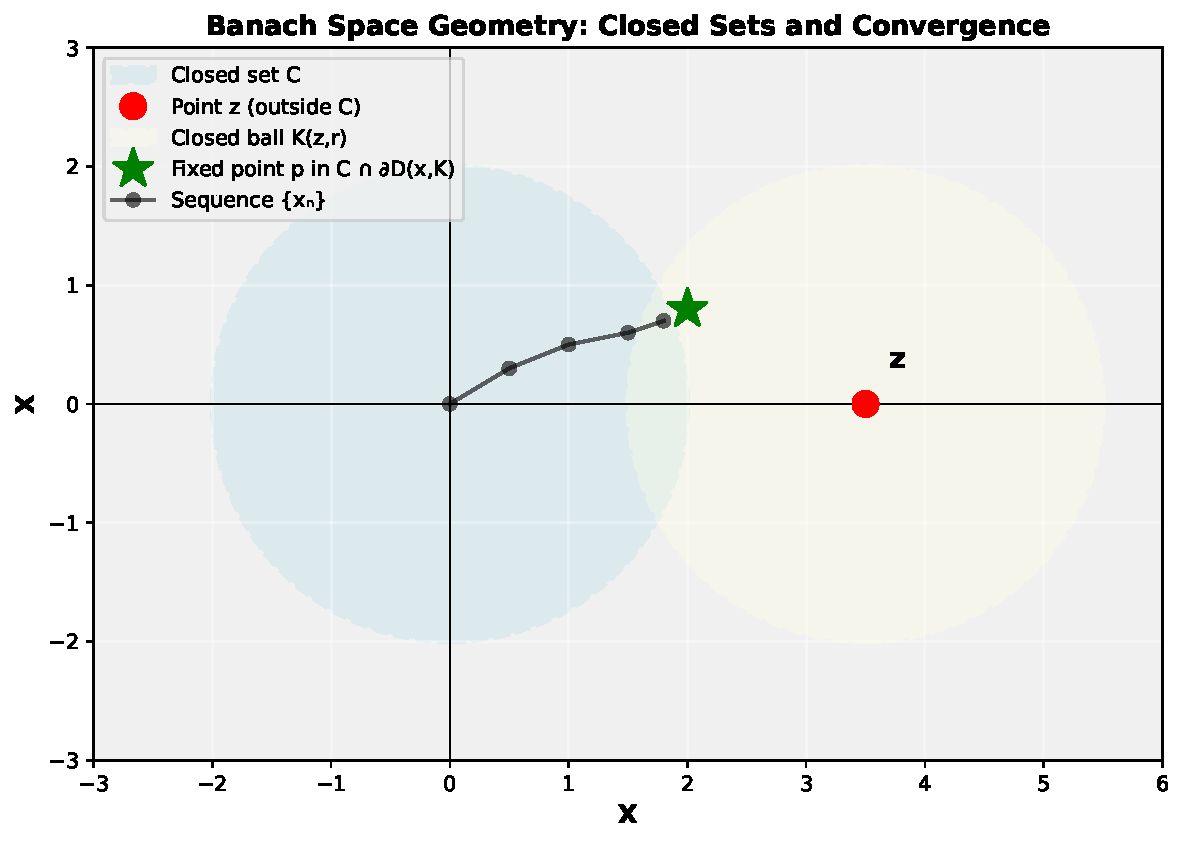
\includegraphics[width=0.8\textwidth]{banach_space_geometry.pdf}
    \end{center}

    The diagram illustrates key geometric concepts:
    \begin{itemize}
        \item Closed set $C$ (blue dashed circle)
        \item External point $z$ and ball $K(z,r)$ (orange)
        \item Convergent sequence and fixed point $p$ (green star)
    \end{itemize}
\end{frame}

% ============================================================================
\section{9.2: Application to System of Linear Equations}
% ============================================================================

\begin{frame}[fragile]{Linear System and Fixed Point Formulation}
    Consider the system of $n$ linear equations:
    \[
    \begin{cases}
    a_{11}x_1 + a_{12}x_2 + \cdots + a_{1n}x_n = b_1 \\
    a_{21}x_1 + a_{22}x_2 + \cdots + a_{2n}x_n = b_2 \\
    \vdots \\
    a_{n1}x_1 + a_{n2}x_2 + \cdots + a_{nn}x_n = b_n
    \end{cases}
    \]

    Rewrite as: $\mathbf{x} = \mathbf{x} - A\mathbf{x} + \mathbf{b}$ where $A = (a_{ij})_{n \times n}$ and $\mathbf{b} = (b_1, \ldots, b_n)^T$.

    \vspace{0.3cm}

    \textbf{Key Idea:} Apply Banach contraction theorem with $T(\mathbf{x}) = \mathbf{x} - A\mathbf{x} + \mathbf{b}$ to find unique solution $\mathbf{x}^*$.

    \vspace{0.3cm}

    \textbf{Convergence Condition:} Spectral radius $\rho(I - A) < 1$ ensures contraction.
\end{frame}

\begin{frame}[fragile]{Linear System: Iterative Algorithm}
    \begin{block}{Jacobi Iteration for Linear Systems}
        Given: Matrix $A$ and vector $\mathbf{b}$, with $a_{ii} \neq 0$.

        \smallskip
        \textbf{Fixed point iteration:}
        \[x_i^{(k+1)} = \frac{1}{a_{ii}}\left(b_i - \sum_{j \neq i} a_{ij} x_j^{(k)}\right), \quad i = 1,2,\ldots,n\]

        \smallskip
        \textbf{Convergence:} If $A$ is diagonally dominant, the iteration converges.
    \end{block}

    \vspace{0.4cm}

    \textbf{Example:} Consider the system
    \[
    \begin{pmatrix} 4 & 1 & 0 \\ 0 & 3 & 1 \\ 0 & 1 & 2 \end{pmatrix}
    \begin{pmatrix} x_1 \\ x_2 \\ x_3 \end{pmatrix}
    =
    \begin{pmatrix} 1 \\ 2 \\ 1 \end{pmatrix}
    \]

    Apply Jacobi iterations starting from $\mathbf{x}^{(0)} = (0,0,0)^T$ to obtain the solution.
\end{frame}

% ============================================================================
\section{9.2.1: Nonlinear Matrix Equations}
% ============================================================================

\begin{frame}{Nonlinear Matrix Equation Problem}
    \begin{block}{Problem Setup}
        Consider the matrix equation:
        \[X = Q + \sum_{i=1}^m A_i X^{\delta_i} A_i^*, \quad 0 < \delta_i < 1\]

        where:
        \begin{itemize}
            \item $Q$ is an $n \times n$ positive semidefinite matrix
            \item $A_i$ are nonsingular $n \times n$ matrices
            \item $X$ is the positive definite solution
        \end{itemize}
    \end{block}

    \vspace{0.3cm}

    \textbf{Applications:} Control theory, stability analysis, and system identification.

    \vspace{0.3cm}

    \textbf{Thompson Metric:} On cone $P(N)$ of Hermitian positive definite matrices:
    \[d(A,B) = \max\{\log M(A/B), \log M(B/A)\}\]
    where $M(A/B) = \lambda_{\max}(B^{-1/2}AB^{-1/2})$ is the maximal eigenvalue.
\end{frame}

\begin{frame}{Theorem 9.8: Convergence to Unique Solution}
    \begin{block}{Theorem 9.8}
        Suppose $\lambda = \max\{|\alpha_1|, |\alpha_2|, \ldots, |\alpha_{r+1}|\} \in (0,1)$ where $\alpha_i$ are real parameters. Then:

        \begin{enumerate}
            \item The equation $X = Q + A_1^* X^{\alpha_1} A_1 + A_2^* X^{\alpha_2} A_2 + \cdots + A_{r+1}^* X^{\alpha_{r+1}} A_{r+1}$ has a \textbf{unique equilibrium point} $U \in P(N)$ satisfying
            \[U = Q + A_1^* U^{\alpha_1} A_1 + A_2^* U^{\alpha_2} A_2 + \cdots + A_{r+1}^* U^{\alpha_{r+1}} A_{r+1}\]

            \item The iterative sequence $\{X_n\}$ defined by the recursion \textbf{converges to the unique solution} of the matrix equation.
        \end{enumerate}
    \end{block}
\end{frame}

\begin{frame}{Numerical Example: Matrix Convergence}
    \begin{center}
        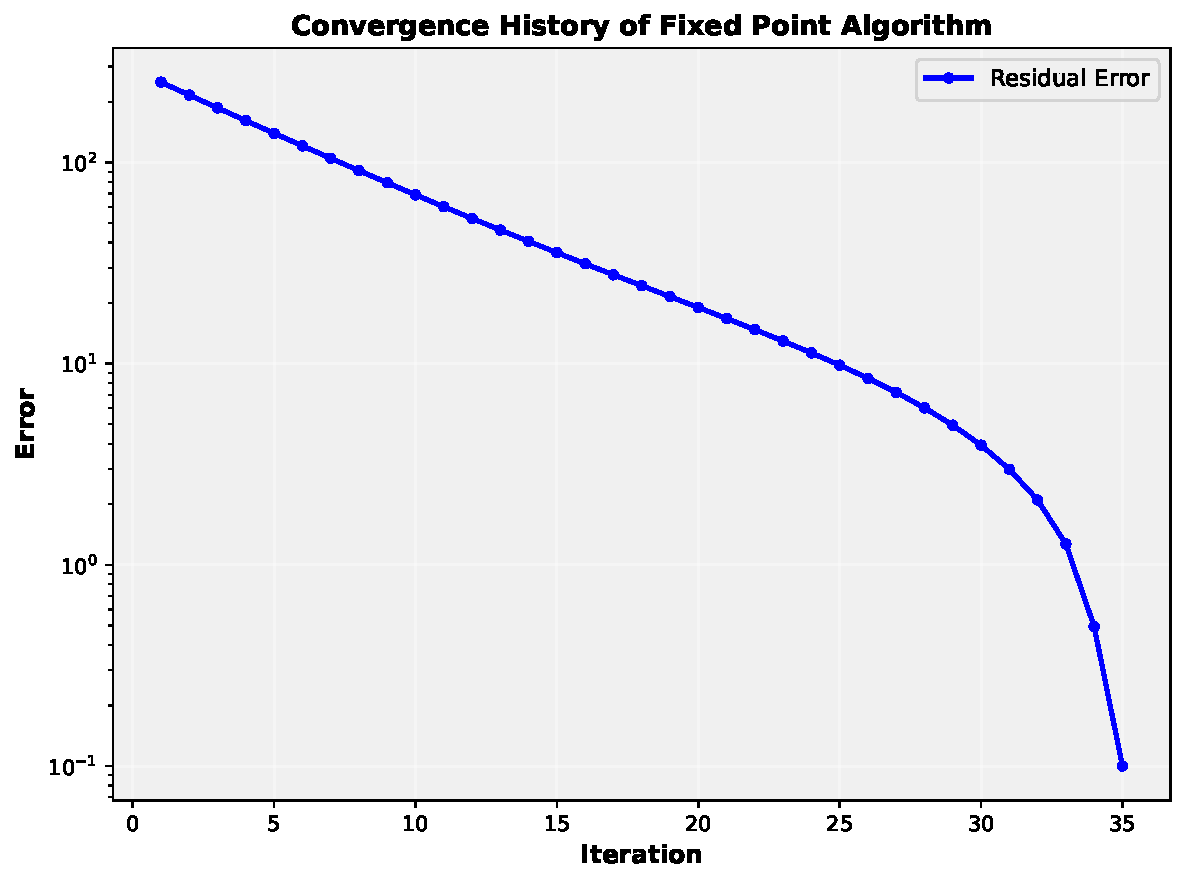
\includegraphics[width=0.85\textwidth]{convergence_history.pdf}
    \end{center}

    \textbf{Convergence History:} After 35 iterations, the sequence converges to the unique positive definite solution
    \[U = X_{35} = \begin{pmatrix} 639.18 & 54.17 & 107.36 \\ 54.13 & 44.78 & 44.15 \\ 104.40 & 42.11 & 112.55 \end{pmatrix}\]
\end{frame}

% ============================================================================
\section{9.3: Application to Control Theory}
% ============================================================================

\begin{frame}{Control Theory: Problem Formulation}
    \begin{block}{Optimal Control Problem}
        Consider the ordinary differential equation (ODE):
        \[\dot{x}(s) = f(x(s), \alpha(s)), \quad x(t) = x_0\]

        where $\alpha(\cdot) \in \mathcal{A}$ is an admissible control.

        \smallskip

        Find optimal control $\alpha^*(\cdot)$ that minimizes the cost functional:
        \[C_{x_0}[\alpha(\cdot)] := \int_t^T h(x(s), \alpha(s))ds + g(x(T))\]
    \end{block}

    \vspace{0.3cm}

    \textbf{Key Components:}
    \begin{itemize}
        \item Running cost: $h(\mathbf{x},\alpha)$ per unit time
        \item Terminal cost: $g(\mathbf{x}(T))$ at final time
        \item Value function: $u(x,t) := \inf_{\alpha \in \mathcal{A}} C_{x,t}[\alpha]$
    \end{itemize}
\end{frame}

\begin{frame}{Control Theory: Value Function and Hamilton-Jacobi PDE}
    \begin{block}{Value Function Properties}
        The value function $u(x,t)$ solves Hamilton-Jacobi PDE:
        \[u_t(x,t) + \inf_{\alpha \in \mathcal{A}} \left\{h(x,\alpha) + \nabla u \cdot f(x,\alpha)\right\} = 0\]
        with terminal condition $u(x,T) = g(x)$.
    \end{block}

    \vspace{0.3cm}

    \begin{block}{Optimality Conditions}
        For each $\xi > 0$ small with $t + \xi \leq T$:
        \[u(x,t) := \inf_{\alpha \in \mathcal{A}} \left\{\int_t^{t+\xi} h(x(s), \alpha(s))ds + u(x(t+\xi), t+\xi)\right\}\]
    \end{block}

    \vspace{0.3cm}

    \textbf{Application:} Dynamic programming approach using fixed point methods on operator equations.
\end{frame}

\begin{frame}{Control System Visualization}
    \begin{center}
        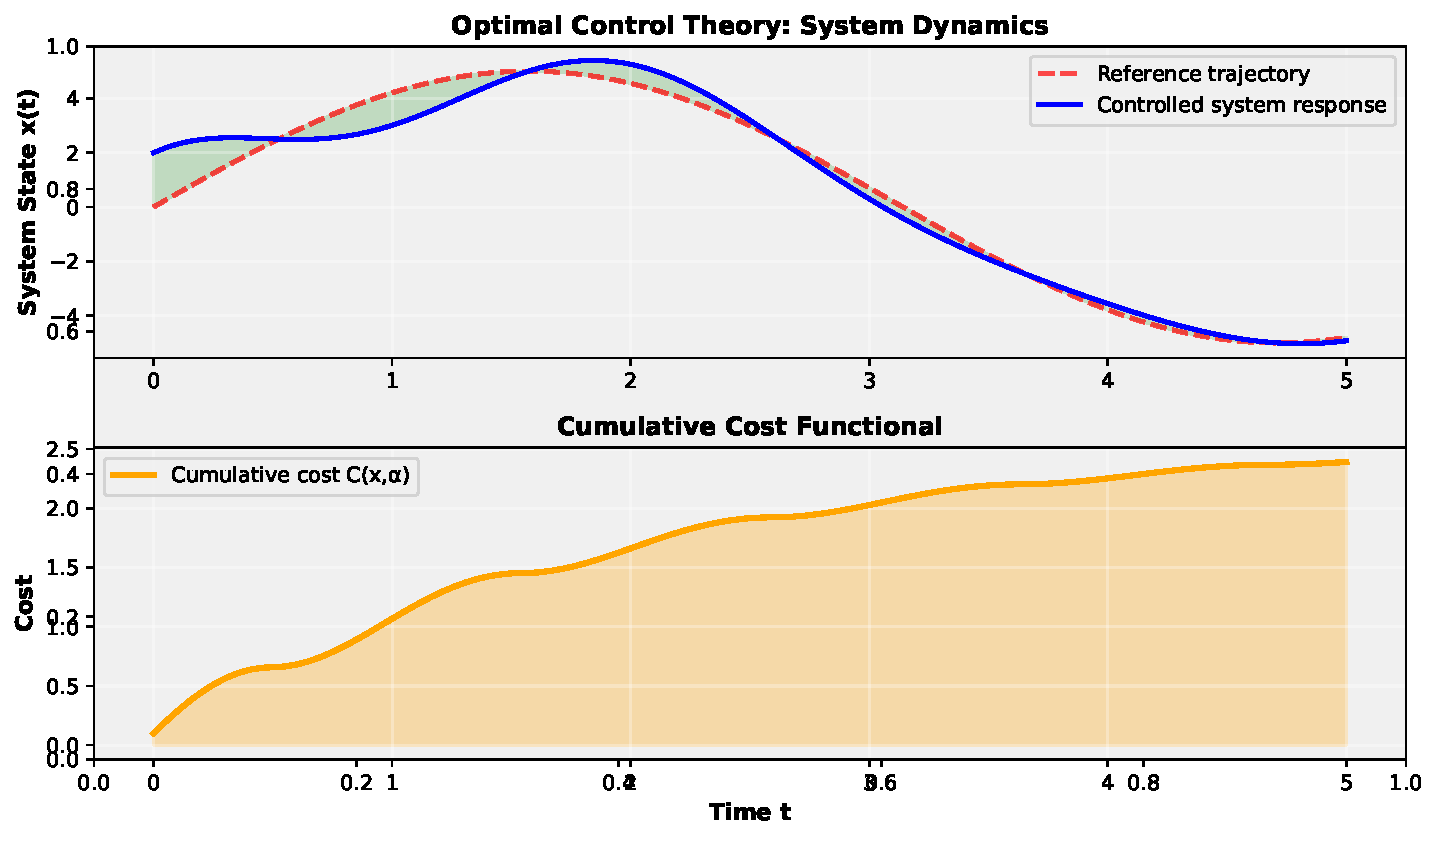
\includegraphics[width=0.95\textwidth]{control_theory_system.pdf}
    \end{center}

    The plots show:
    \begin{itemize}
        \item \textbf{Top:} Reference trajectory vs. controlled system response
        \item \textbf{Bottom:} Cumulative cost functional showing optimality
    \end{itemize}
\end{frame}

% ============================================================================
\section{9.3.1: Variational Inequalities}
% ============================================================================

\begin{frame}{Variational Inequalities in Stochastic Control}
    \begin{block}{Two-Obstacle Variational Inequality}
        Find function $u$ such that:
        \[\max\{\min\{Lu - f, u - \phi\}, u - \mu\} = 0 \quad \text{on } \Omega\]
        with boundary condition $u = 0$ on $\partial\Omega$.

        \smallskip

        Here:
        \begin{itemize}
            \item $L = -a_{ij}(x)\frac{\partial^2}{\partial x_i \partial x_j} + b_i(x)\frac{\partial}{\partial x_i} + c(x)I_N$ is elliptic operator
            \item $\phi < \mu$ are obstacle functions
            \item Solution must lie in feasible region $[\mu, \phi]$
        \end{itemize}
    \end{block}

    \vspace{0.3cm}

    \textbf{Interpretation:} Two competing controls; the solution reflects optimal play.
\end{frame}

\begin{frame}{M-Matrix and Discrete Variational Inequality}
    \begin{definition}{M-matrix}
        A square matrix $A$ is an M-matrix if and only if every off-diagonal entry is nonpositive.
    \end{definition}

    \vspace{0.3cm}

    \begin{block}{Discrete Two-Obstacle Problem}
        For discrete case with B-matrix $B = I_N - A$:
        \[\max\{\min\{A(x - A^*d(x, Tx)) - f, x - A^*d(x, Tx) - \phi\}, x - A^*d(x, Tx) - \mu\} = 0\]

        where $T$ is defined implicitly by the min-max conditions.
    \end{block}

    \vspace{0.3cm}

    \begin{block}{Theorem 9.9}
        Under assumptions (9.27) and (9.28) on matrices, a solution to equation (9.31) exists.
    \end{block}
\end{frame}

\begin{frame}{Variational Inequality Visualization}
    \begin{center}
        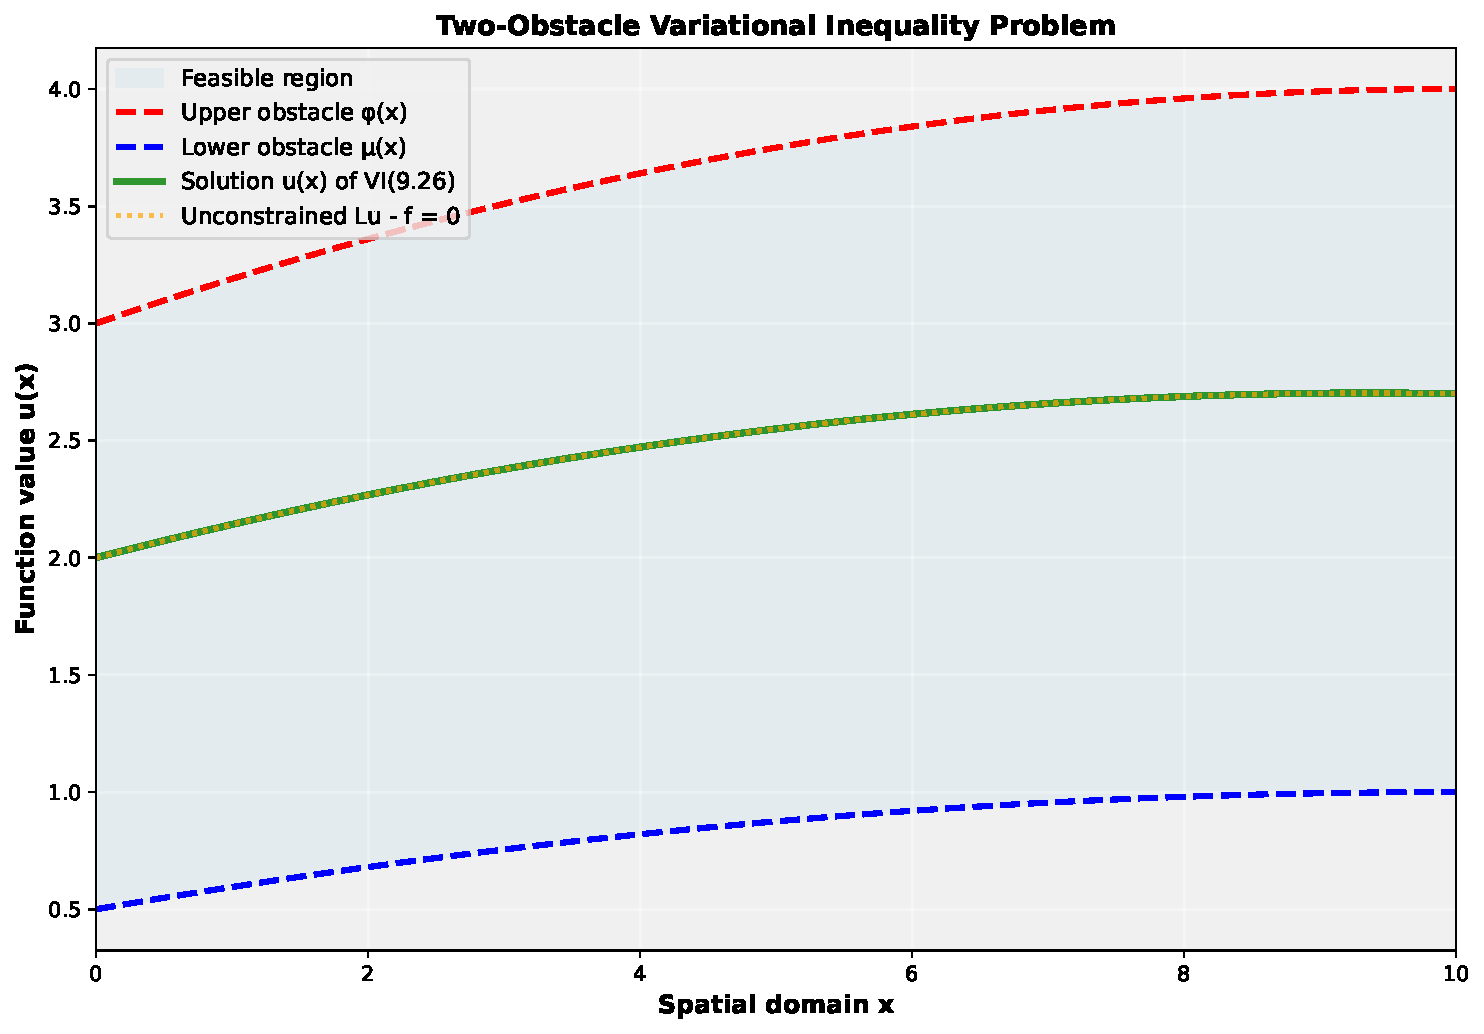
\includegraphics[width=0.95\textwidth]{variational_inequality.pdf}
    \end{center}

    The solution $u(x)$ respects both obstacles while minimizing the cost of solving $Lu = f$.
\end{frame}

% ============================================================================
\section{9.3.2: Game Theory and Nash Equilibria}
% ============================================================================

\begin{frame}{Two-Person Zero-Sum Game}
    \begin{definition}{Nash Equilibrium}
        A pair of strategies $(x^*, y^*) \in \triangle^m \times \triangle^n$ (simplices) is a Nash equilibrium if:
        \begin{align*}
        e_1(x, y^*) &\leq e_1(x^*, y^*), \quad \text{for all } x \in \triangle^m \\
        e_2(x^*, y) &\leq e_2(x^*, y^*), \quad \text{for all } y \in \triangle^n
        \end{align*}

        where $e_i(\mathbf{x}, \mathbf{y})$ are expected payoff functions for players 1 and 2.
    \end{definition}

    \vspace{0.3cm}

    \textbf{Key Properties:}
    \begin{itemize}
        \item $(x^*, y^*)$ is a fixed point of the best-response mapping
        \item Neither player can unilaterally improve payoff by changing strategy
        \item Probability-based mixed strategies determine average outcomes
    \end{itemize}

    \vspace{0.3cm}

    \textbf{Expected Payoffs:} For payoff matrix $P = (p_{ij})$:
    \begin{align*}
    e_1(\mathbf{x}, \mathbf{y}) &= \mathbf{x}P\mathbf{y}^T = \sum_{i=1}^m \sum_{j=1}^n x_i y_j p_{ij}
    \end{align*}
\end{frame}

\begin{frame}{Theorem 9.10: Existence of Nash Equilibrium}
    \begin{block}{Theorem 9.10 (Fundamental Theorem of Game Theory)}
        \textbf{For a two-player zero-sum game, there exists a Nash equilibrium.}

        \vspace{0.3cm}

        \textit{Proof Sketch:}
        \begin{enumerate}
            \item The space of all pairs $(\mathbf{x}, \mathbf{y})$ is homeomorphic to $(m+n)$-dimensional disc $\triangle^m \times \triangle^n$
            \item Define continuous mapping $g: \triangle^m \times \triangle^n \to \triangle^m \times \triangle^n$ where fixed point represents Nash equilibrium
            \item Apply Brouwer's fixed point theorem to guarantee existence
            \item The fixed point satisfies all equilibrium conditions
        \end{enumerate}
    \end{block}

    \vspace{0.3cm}

    \textbf{Conclusion:} Every finite two-person zero-sum game has at least one Nash equilibrium (possibly in mixed strategies).
\end{frame}

\begin{frame}{Nash Equilibrium Payoff Analysis}
    \begin{center}
        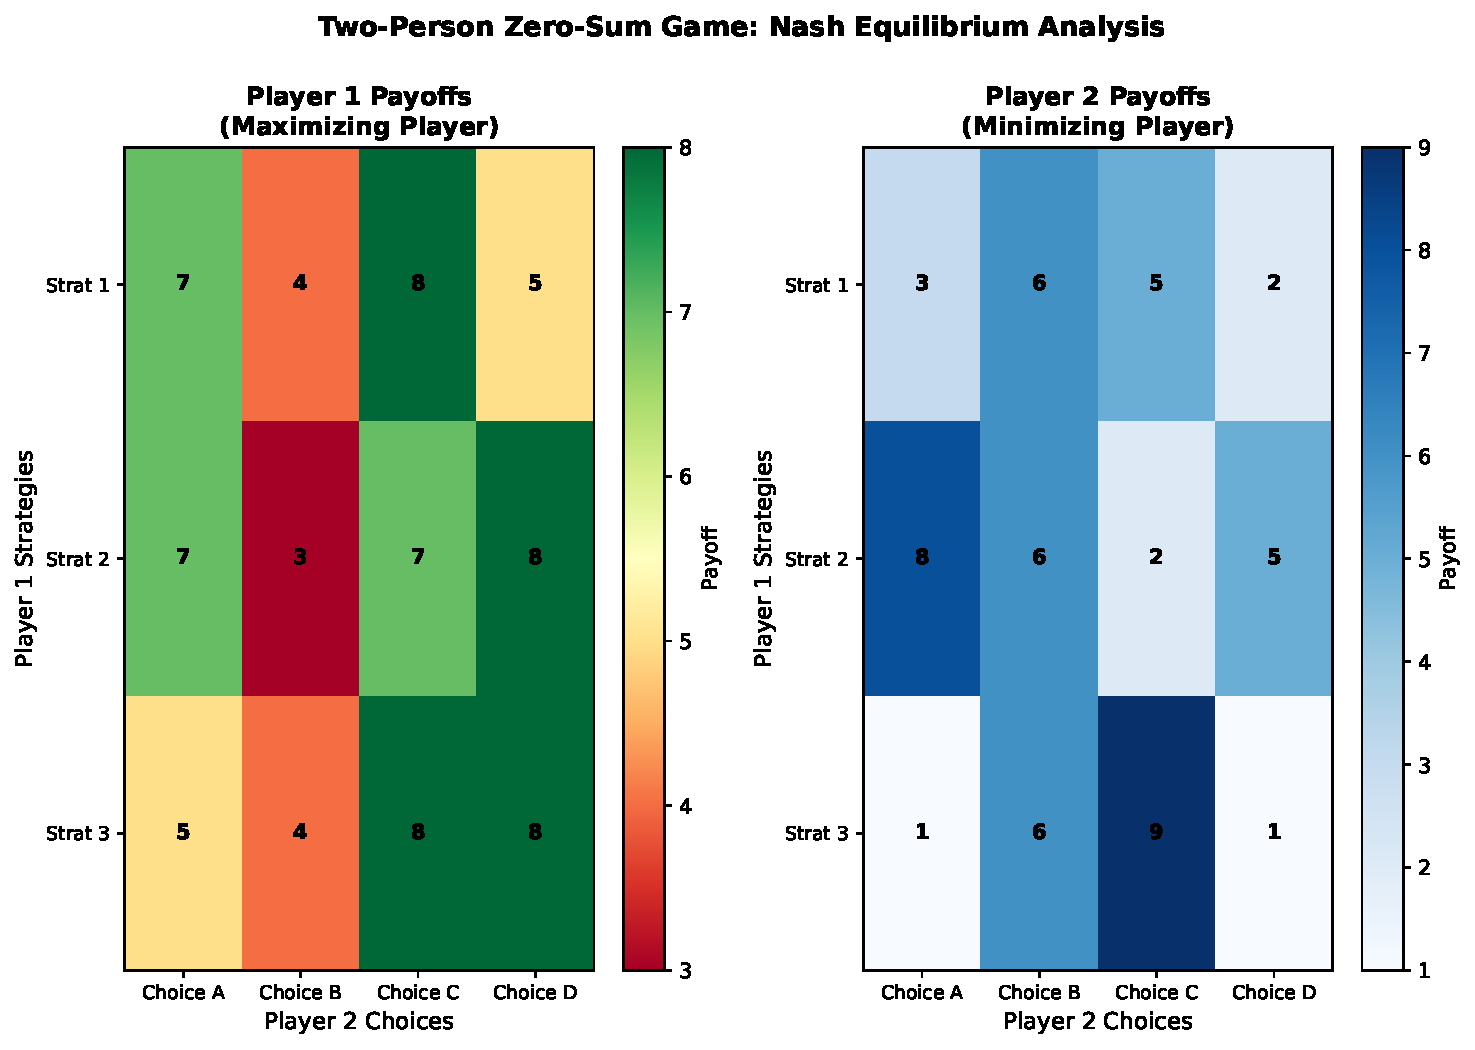
\includegraphics[width=0.95\textwidth]{nash_equilibrium.pdf}
    \end{center}

    The heatmaps show the strategic landscape for both players:
    \begin{itemize}
        \item \textbf{Left (Player 1):} Maximizing player seeks high payoffs
        \item \textbf{Right (Player 2):} Minimizing player seeks low payoffs for opponent
        \item Nash equilibrium found where best-responses intersect
    \end{itemize}
\end{frame}

% ============================================================================
\section{9.4: Application to Differential Equations}
% ============================================================================

\begin{frame}{9.4.1: Picard-Lindelof Existence Theorem}
    \begin{block}{Theorem 9.11 (Picard-Lindelof)}
        Let $\Omega$ denote an open set in $\mathbb{R}^2$, $(t_0, x_0) \in \Omega$. Let $f(t,x)$ be real-valued, continuous in $\Omega$, and satisfy the Lipschitz condition
        \[|f(t, x_1) - f(t, x_2)| \leq M|x_1 - x_2|, \quad (t,x_1), (t,x_2) \in \Omega\]

        Then there exists $\tau > 0$ and a unique function $\varphi(t)$ continuous and differentiable in $[t_0 - \tau, t_0 + \tau]$ such that:
        \begin{enumerate}
            \item $\varphi(t_0) = x_0$
            \item $\dot{x}(t) = f(t, x(t))$ for $t \in [t_0 - \tau, t_0 + \tau]$
        \end{enumerate}
    \end{block}

    \vspace{0.3cm}

    \textbf{Proof Strategy:} Reduce ODE to Hammerstein integral equation, then apply Banach contraction theorem on appropriate function space.
\end{frame}

\begin{frame}[fragile]{Picard-Lindelof: Integral Formulation}
    \begin{block}{Reduction to Integral Equation}
        The ODE $\dot{x}(t) = f(t, x(t))$ with initial condition $x(t_0) = x_0$ is equivalent to:
        \[\varphi(t) = x_0 + \int_{t_0}^t f(s, \varphi(s)) ds\]
    \end{block}

    \vspace{0.3cm}

    \begin{block}{Contraction Mapping on $E = C[t_0 - \tau, t_0 + \tau]$}
        Define metric space $(E, \|\cdot\|)$ where $\|u\| = \max_{t \in [t_0-\tau, t_0+\tau]} |u(t)|$.

        \smallskip

        Define $\Psi: E \to E$ by
        \[\Psi(u)(t) = x_0 + \int_{t_0}^t f(s, u(s)) ds\]

        \smallskip

        For $\tau m < 1$ (where $m$ is upper bound of $|f|$), $\Psi$ is contraction with unique fixed point.
    \end{block}

    \vspace{0.3cm}

    \textbf{Key:} Fixed point of $\Psi$ is the unique solution to the ODE.
\end{frame}

\begin{frame}[fragile]{Differential Equation Example}
    \begin{block}{Example: Linear First-Order ODE}
        Solve $\dot{x}(t) = \lambda x(t)$ with $x(0) = x_0$ using fixed point method.

        \vspace{0.3cm}

        The integral equation becomes:
        \[\varphi(t) = x_0 + \int_0^t \lambda \varphi(s) ds\]

        \vspace{0.3cm}

        Successive approximations:
        \begin{align*}
        \varphi_0(t) &= x_0 \\
        \varphi_1(t) &= x_0 + \int_0^t \lambda x_0 ds = x_0(1 + \lambda t) \\
        \varphi_2(t) &= x_0 + \int_0^t \lambda x_0(1 + \lambda s) ds = x_0\left(1 + \lambda t + \frac{(\lambda t)^2}{2!}\right) \\
        \varphi_n(t) &\to x_0 e^{\lambda t} \quad \text{as } n \to \infty
        \end{align*}
    \end{block}

    \vspace{0.2cm}

    This recovers the classical solution!
\end{frame}

\begin{frame}{Theorem 9.12: Convergence of Successive Approximations}
    \begin{block}{Theorem 9.12}
        If $\varphi_n$ is the solution of the differential equation (9.39) with initial condition $\varphi_n(t_0) = x_0$ and $\{x_n\}$ is a real sequence converging to $x_0$, then $\{\varphi_n\}$ converges to the solution $\varphi$ of (9.39) with $\varphi(t_0) = x_0$ in $E$.

        \vspace{0.3cm}

        \textit{Proof:} The Picard iterates form a Cauchy sequence in the complete metric space $C[t_0-\tau, t_0+\tau]$, converging to the unique fixed point of the contraction mapping.
    \end{block}

    \vspace{0.3cm}

    \textbf{Practical Significance:} Allows numerical solution via iterative computation of successive approximations.
\end{frame}

\begin{frame}{Fixed Point Iteration Method}
    \begin{center}
        
\includegraphics[width=0.95\textwidth]{fixed_point_iteration.pdf}
    \end{center}

    Graphical method for finding fixed point $x^*$ where the curve $y = T(x)$ intersects the line $y = x$.
\end{frame}

% ============================================================================
\section{Summary and Conclusions}
% ============================================================================

\begin{frame}{Key Takeaways}
    \begin{columns}[T]
        \column{0.5\textwidth}
        \begin{block}{Theory Highlights}
            \begin{itemize}
                \item Banach contraction theorem extends to approximation problems
                \item Convergence depends on metric structure and contraction ratios
                \item Applications span diverse fields: linear/nonlinear systems, control, game theory
            \end{itemize}
        \end{block}

        \column{0.5\textwidth}
        \begin{block}{Practical Applications}
            \begin{itemize}
                \item Solving large-scale matrix equations
                \item Optimal control and dynamic programming
                \item Game-theoretic equilibrium computation
                \item Existence proofs for PDEs and ODEs
            \end{itemize}
        \end{block}
    \end{columns}

    \vspace{0.5cm}

    \begin{block}{Unifying Principle}
        All applications use the same core technique: reduce the problem to finding a fixed point of a contraction mapping, then invoke the Banach contraction theorem to guarantee existence, uniqueness, and convergence.
    \end{block}
\end{frame}

\begin{frame}{Convergence Rates and Computational Complexity}
    \begin{columns}[T]
        \column{0.5\textwidth}
        \begin{block}{Linear Convergence}
            \[d(x_n, x^*) \leq \lambda^n d(x_0, x^*)\]

            \smallskip

            Convergence factor $\lambda = \max\{|\alpha_i|\}$:
            \begin{itemize}
                \item $\lambda < 0.5$: Fast convergence
                \item $0.5 < \lambda < 1$: Moderate convergence
                \item $\lambda$ close to 1: Slow convergence
            \end{itemize}
        \end{block}

        \column{0.5\textwidth}
        \begin{block}{Practical Considerations}
            \begin{itemize}
                \item Iteration count $n^*$ for tolerance $\epsilon$: \[n^* \approx \frac{\ln(\epsilon/d_0)}{\ln \lambda}\]
                \item Trade-off: simple iteration vs. complicated fixed point operator
                \item Preconditioners improve contraction ratio
            \end{itemize}
        \end{block}
    \end{columns}

    \vspace{0.5cm}

    \begin{center}
        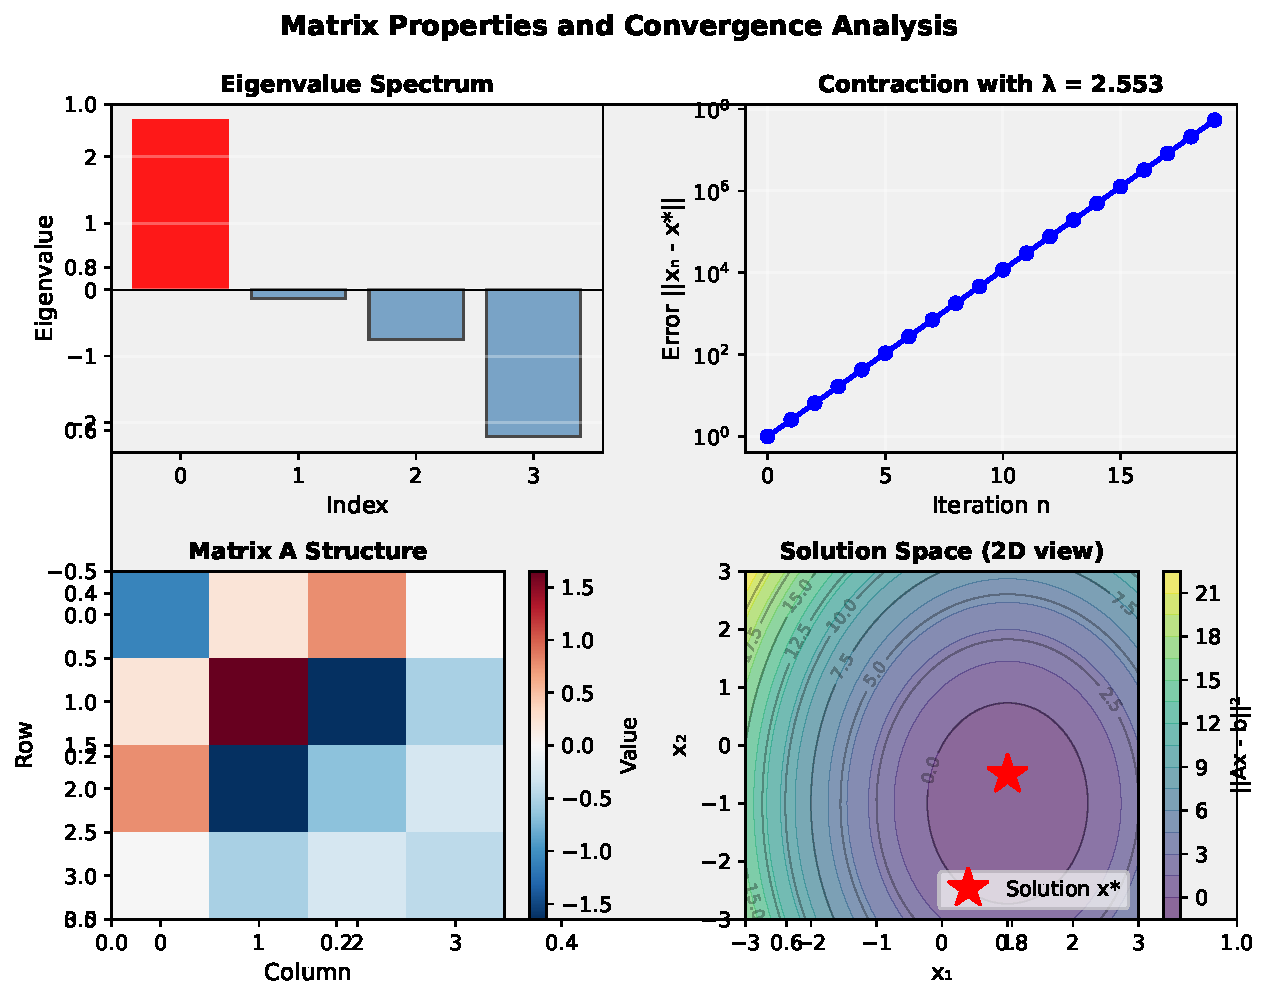
\includegraphics[width=0.8\textwidth]{matrix_eigenvalues.pdf}
    \end{center}
\end{frame}

\begin{frame}[fragile]{Python Implementation Example}
    \begin{lstlisting}[language=Python, basicstyle=\ttfamily\tiny]
import numpy as np

def fixed_point_iteration(T, x0, tol=1e-6, max_iter=1000):
    """
    Fixed point iteration: x_{n+1} = T(x_n)
    """
    x = x0.copy()
    errors = []

    for n in range(max_iter):
        x_new = T(x)
        error = np.linalg.norm(x_new - x)
        errors.append(error)

        if error < tol:
            print(f"Converged in {n} iterations")
            return x_new, errors

        x = x_new

    print(f"Max iterations reached: {max_iter}")
    return x, errors

# Example: Solve linear system Ax = b via T(x) = x - Ax + b
A = np.array([[2, 0.5], [0.5, 2]])
b = np.array([1, 1])
x0 = np.zeros(2)

T = lambda x: x - A @ x + b
solution, errors = fixed_point_iteration(T, x0)
print(f"Solution: {solution}")
    \end{lstlisting}
\end{frame}

\begin{frame}{Future Extensions and Research Directions}
    \begin{itemize}
        \item \textbf{Nonlinear Operators:} Extension to monotone operators and variational inequalities
        \item \textbf{Higher-Dimensional Systems:} Scaling and parallelization for large-scale problems
        \item \textbf{Adaptive Methods:} Dynamic contraction rates based on computed residuals
        \item \textbf{Machine Learning:} Neural network approximations of fixed point mappings
        \item \textbf{Hybrid Methods:} Combining fixed point iterations with gradient-based optimization
    \end{itemize}

    \vspace{0.5cm}

    \textbf{References:}
    \begin{itemize}
        \item Pathak, H. K. (2009). \textit{An Introduction to Nonlinear Analysis and Fixed Point Theory}
        \item Banach, S. (1922). Sur les opérations dans les ensembles abstraits et leur application aux équations intégrales
        \item Caristi, J. (1976). Fixed point theorems for mappings satisfying inwardness conditions
    \end{itemize}
\end{frame}

\end{document}
